% Slides --- artigo (IaC + Data Lake no OCI Free Tier); compilar com CWD = esta pasta
\documentclass[aspectratio=169,11pt]{beamer}

\usetheme{cefetmg}
\graphicspath{{../content/assets/}}

\hypersetup{
  colorlinks=true,
  linkcolor=cefetPrimary!80!black,
  urlcolor=cefetAccent,
  citecolor=cefetAccent,
  pdftitle={Apresentacao - Data Lake Hadoop no OCI Free Tier (IaC)},
  pdfauthor={Joao Pedro Ferreira Duarte}
}

\title[Data Lake IaC no OCI Free Tier]{An Infrastructure-as-Code Framework for Deploying Hadoop Data Lakes on Free-Tier ARM Cloud Instances}
\author[JP Duarte]{Jo\~ao Pedro Ferreira Duarte}
\institute[Cefet Data Platform]{%
  Infraestrutura como c\'odigo, ARM na Oracle Cloud (Free Tier) e avalia\c{c}\~ao com Star Schema Benchmark.\\[0.35em]
  {\mdseries Campus Tim\'oteo --- Engenharia de Computa\c{c}\~ao (CEFET-MG)}%
}
\date{2026}

\institutionhead{%
  Centro Federal de Educa\c{c}\~ao Tecnol\'ogica de Minas Gerais\\[0.15em]
  {\mdseries Campus Tim\'oteo}\\[0.1em]
  {\mdseries Gradua\c{c}\~ao em Engenharia de Computa\c{c}\~ao}%
}
\orientadorlinha{Evandrino Gomes Barros}

\AtBeginSection[]{\cefetSectionFrame}

\begin{document}

\begin{frame}[plain,noframenumbering]
  \titlepage
\end{frame}

\begin{frame}{Sum\'ario}
  \tableofcontents
\end{frame}

\section{Contexto e contribui\c{c}\~oes}
% Contexto e contribuições (~2 min)

\begin{frame}{Motiva\c{c}\~ao}
  \begin{itemize}
    \item Plataformas de Big Data costumam exigir \textbf{infraestrutura cara} e licenciamento, com barreira alta para pesquisa e pequenas organiza\c{c}\~oes.
    \item Mesmo em nuvem, \textbf{custos recorrentes} de clusters multi-n\'o limitam laborat\'orios com or\c{c}amento reduzido.
    \item O \textbf{Oracle Cloud Infrastructure (OCI) Free Tier} oferece inst\^ancias \textbf{ARM Ampere A1} sem custo monet\'ario, por\'em com \textbf{teto severo} de CPU e RAM.
    \item \textbf{Lacuna}: pouca evid\^encia publicada de um pipeline \textbf{IaC ponta a ponta} que provisione e configure um \textbf{Data Lake Hadoop} nesse cen\'ario.
  \end{itemize}
\end{frame}

\begin{frame}{Contribui\c{c}\~oes deste artigo}
  \begin{enumerate}
    \item \textbf{Pipeline IaC} (Terraform + Ansible + Apache Ambari) que cria e configura um cluster de \textbf{4 n\'os} ODP/Hadoop no Free Tier, com \textbf{perfis de instala\c{c}\~ao} configur\'aveis.
    \item \textbf{Avalia\c{c}\~ao emp\'irica} com \textbf{Star Schema Benchmark} (SSB): compara\c{c}\~ao \textbf{Hive vs.\ Spark vs.\ Spark com cache}, sobre ARM fortemente limitado.
    \item \textbf{An\'alise de cache} sob RAM insuficiente para o maior fato ($\sim$9{,}3~GB): quando o cache \textbf{prejudica} ou \textbf{ajuda} o tempo de consulta.
    \item \textbf{Protocolo reprodut\'ivel} e artefatos abertos, vi\'aveis a \textbf{custo zero} em termos de inst\^ancias Free Tier.
  \end{enumerate}
\end{frame}


\section{Arquitetura e implanta\c{c}\~ao}
% Arquitetura e implantação

\begin{frame}{Topologia na OCI (4 n\'os ARM)}
  \begin{itemize}
    \item Um \textbf{mestre} e tr\^es \textbf{workers}; \texttt{VM.Standard.A1.Flex}: \textbf{1 OCPU + 6~GB RAM}/n\'o (4 OCPU / 24~GB agregados).
    \item Oracle Linux 9 \textbf{aarch64}; volumes para HDFS/logs.
    \item \textbf{Security list}: portas \`a Internet restritas ao necess\'ario (Ambari, Hive JDBC, Spark History, \ldots).
  \end{itemize}
\end{frame}

\begin{frame}[plain,t]{Topologia na OCI (diagrama)}
  \vspace{-0.65em}
  {\scriptsize Quatro VMs na sub-rede; \textit{security list}, gateway e volumes para o cluster.\par}
  \vspace{0.12em}
  \centering
  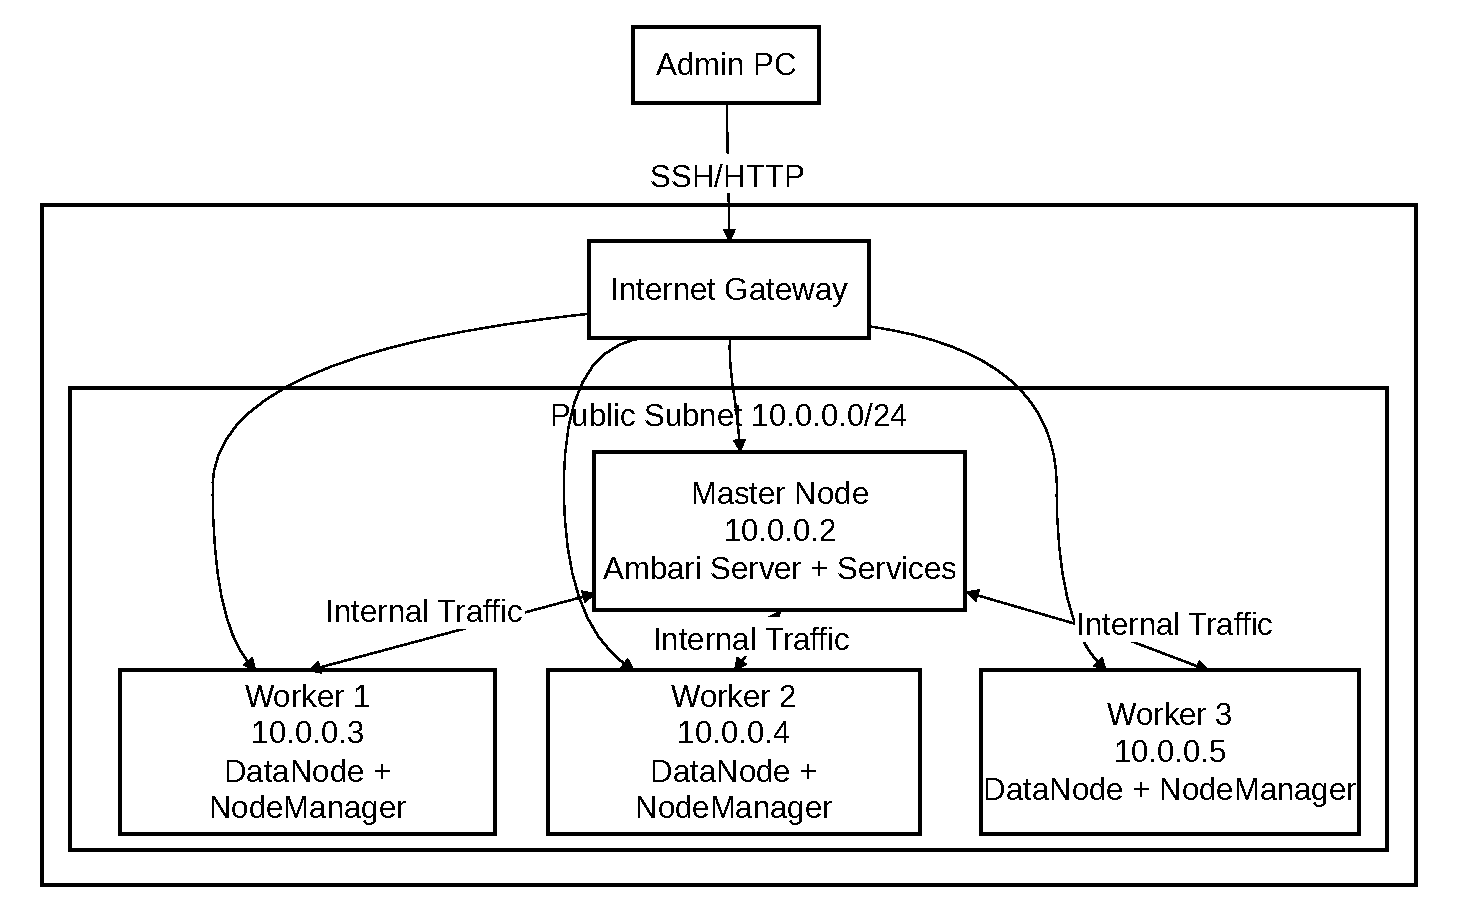
\includegraphics[width=\linewidth,height=0.70\textheight,keepaspectratio]{topology.pdf}
\end{frame}

\begin{frame}{Pipeline automatizado: fase 1 (Terraform)}
  \begin{itemize}
    \item Vari\'aveis: IPs permitidos, perfil; \texttt{terraform apply}.
    \item Rede + 4 inst\^ancias; envia Ansible e scripts Ambari ao mestre.
  \end{itemize}
\end{frame}

\begin{frame}[plain,t]{Fase 1: provisionamento (Terraform)}
  \vspace{-0.65em}
  {\scriptsize Rede (VCN, subnet, \textit{security list}, gateway), chaves TLS, quatro inst\^ancias e c\'opia de playbooks/scripts para o mestre.\par}
  \vspace{0.12em}
  \centering
  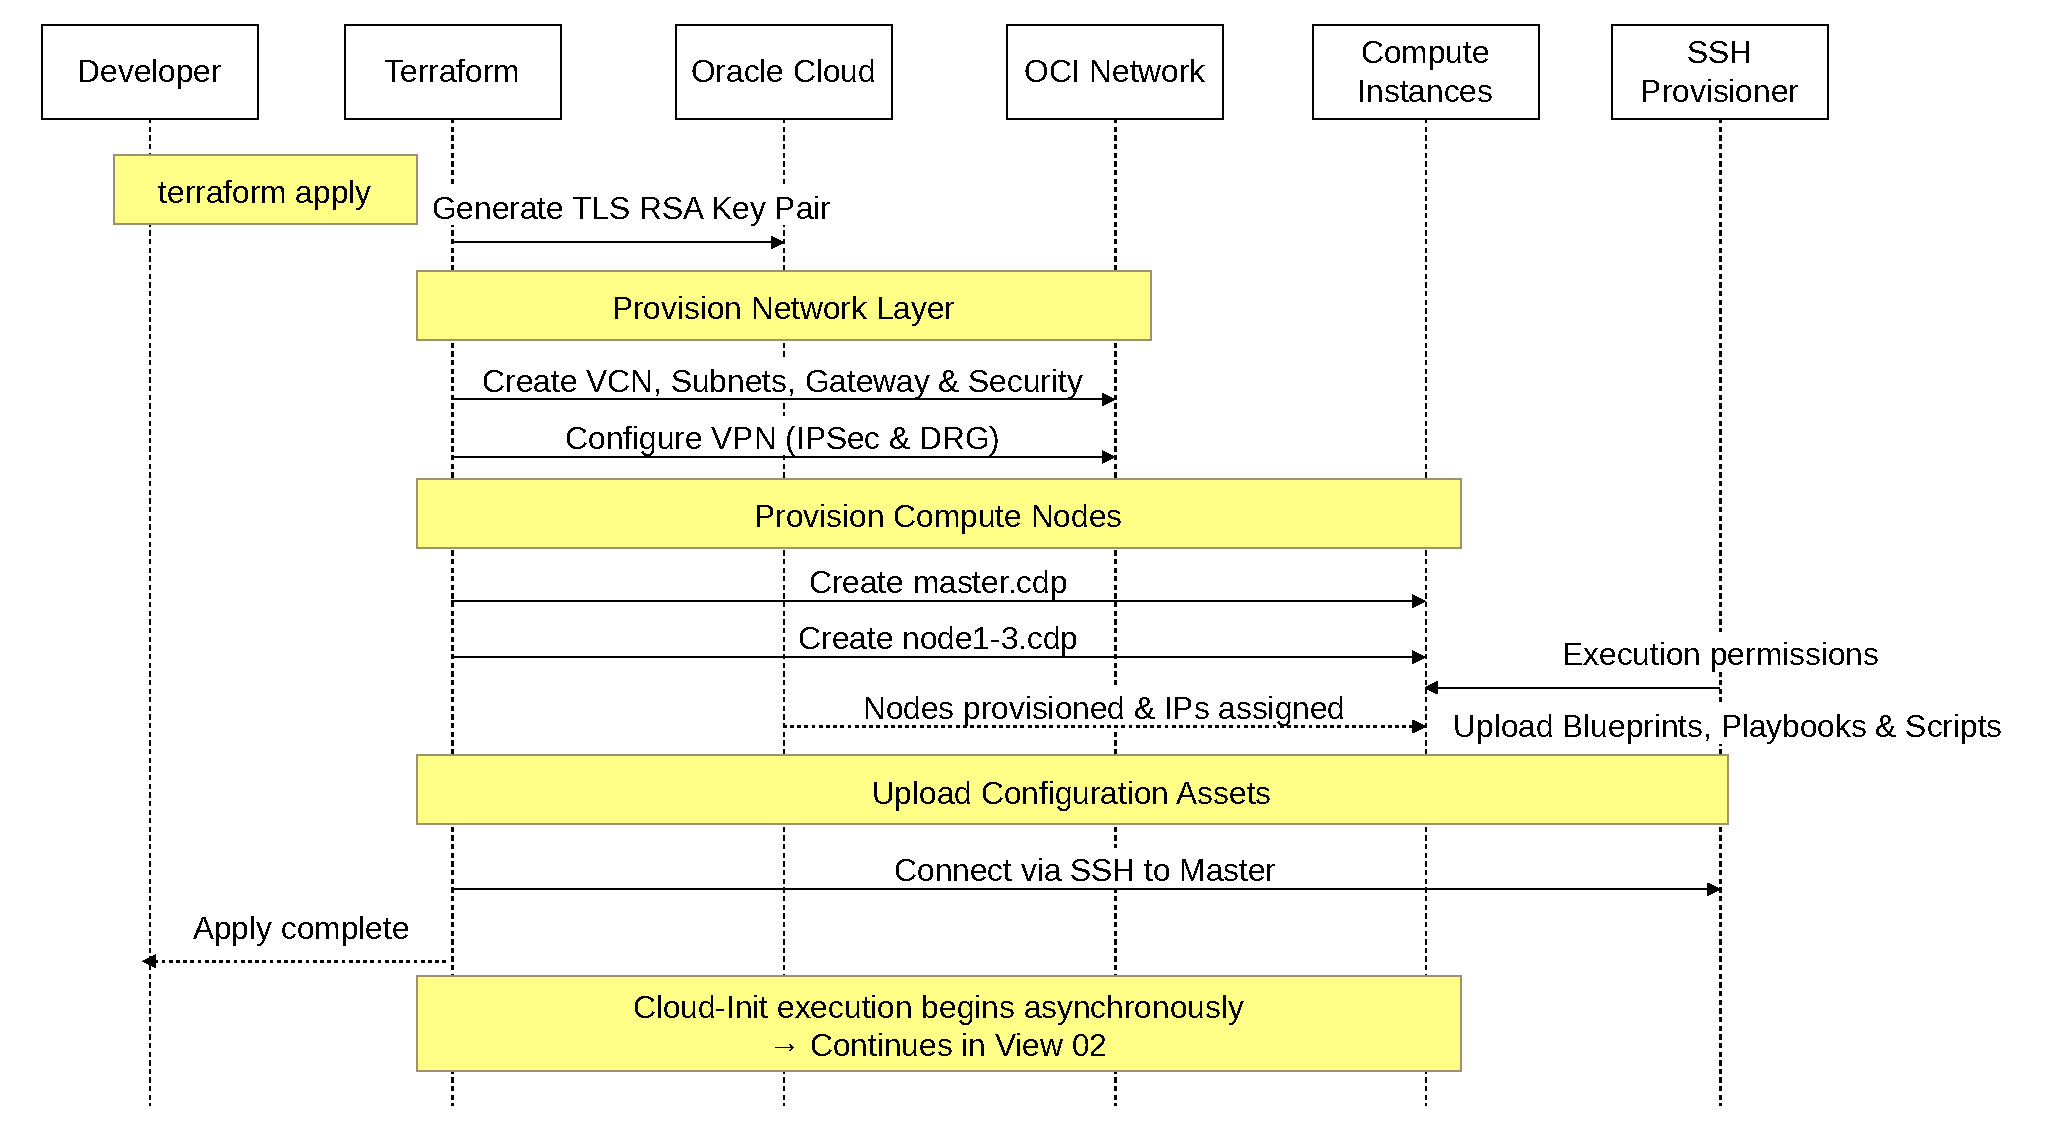
\includegraphics[width=\linewidth,height=0.70\textheight,keepaspectratio]{provisioning-01-terraform.pdf}
\end{frame}

\begin{frame}[plain,t]{Fase 2: SO e pr\'e-requisitos (cloud-init + Ansible)}
  \vspace{-0.6em}
  {\scriptsize Python/Ansible no mestre, \texttt{/etc/hosts}, JDK~8, chrony, PostgreSQL, Ambari Server/Agents\par}
  \vspace{0.15em}
  \centering
  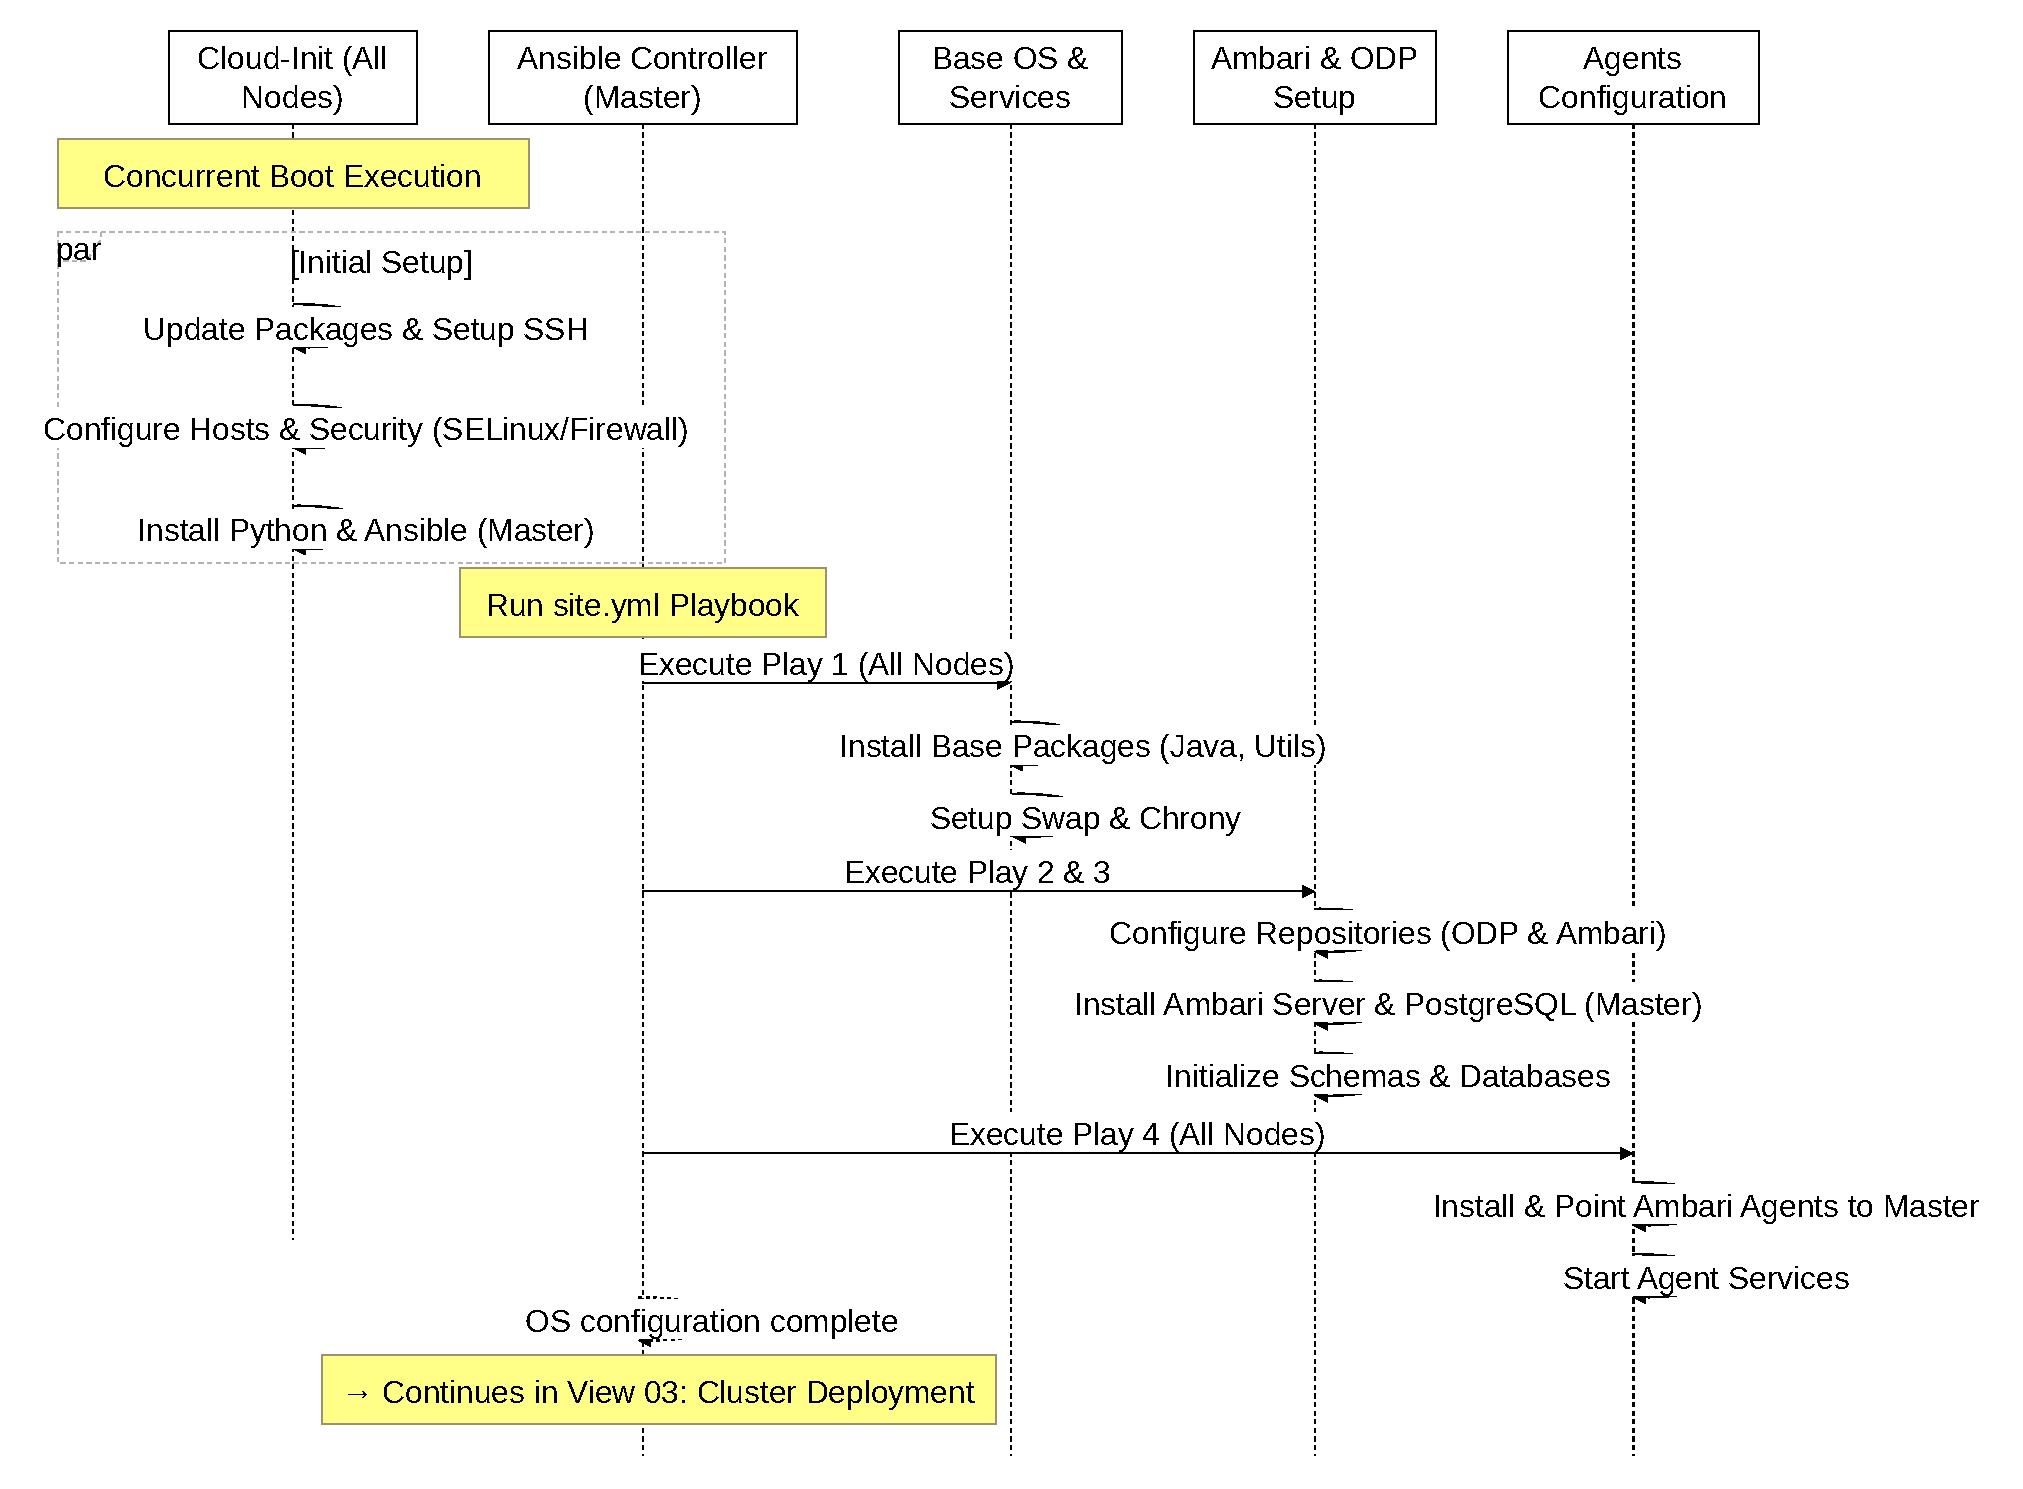
\includegraphics[width=\linewidth,height=0.73\textheight,keepaspectratio]{provisioning-02-os.pdf}
\end{frame}

\begin{frame}[plain,t]{Fase 3: cluster ODP via Ambari (API REST + recupera\c{c}\~ao)}
  \vspace{-0.6em}
  {\scriptsize Blueprint JSON, cria\c{c}\~ao do cluster, ODP~1.2.2.0; recupera\c{c}\~ao autom\'atica (at\'e 3 tentativas)\par}
  \vspace{0.15em}
  \centering
  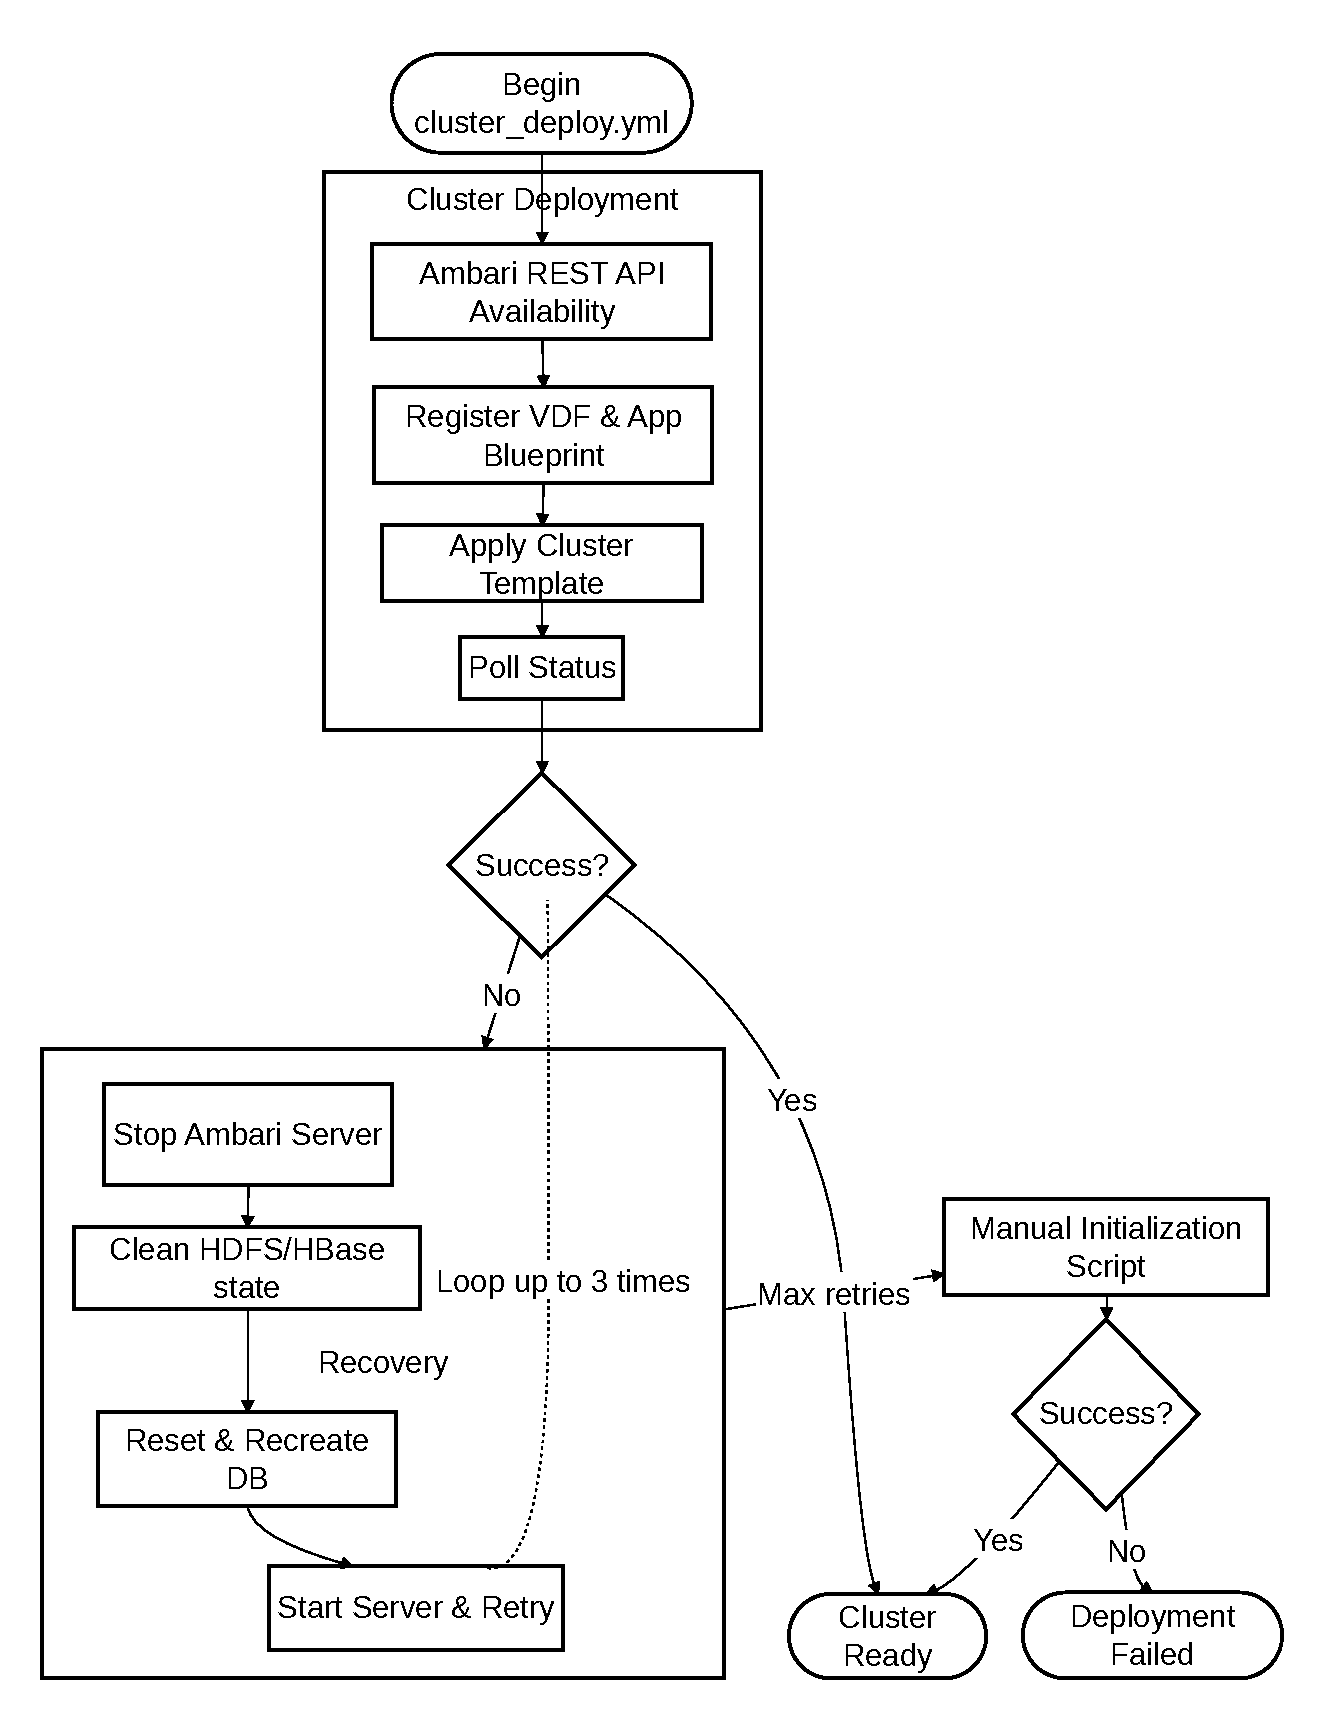
\includegraphics[width=\linewidth,height=0.73\textheight,keepaspectratio]{provisioning-03-cluster.pdf}
\end{frame}

\begin{frame}[shrink=5]{Data Lake em camadas (ODP + Ambari)}
  \small
  \begin{itemize}
    \item \textbf{Ingest\~ao}: Kafka para \textit{streaming}; NiFi para fluxos com \textit{back-pressure} e proveni\^encia; NFS Gateway para ingest\~ao em lote sem clientes Hadoop nos produtores.
    \item \textbf{Armazenamento}: HDFS replicado (blocos 128~MB); HBase para acesso NoSQL de baixa lat\^encia; Hive Metastore como cat\'alogo partilhado por Hive e Spark.
    \item \textbf{Processamento}: YARN agenda contentores; Spark~3 para anal\'itica em mem\'oria; Tez como motor DAG do Hive; HiveServer2 como SQL sobre dados no HDFS.
    \item \textbf{Governan\c{c}a e opera\c{c}\~ao}: Ranger (RBAC, mascaramento, auditoria via Solr); ZooKeeper para coordena\c{c}\~ao; Ambari para ciclo de vida e monitoriza\c{c}\~ao do stack.
  \end{itemize}
\end{frame}

\begin{frame}[plain,t]{Arquitetura em camadas (diagrama)}
  \vspace{-0.55em}
  \centering
  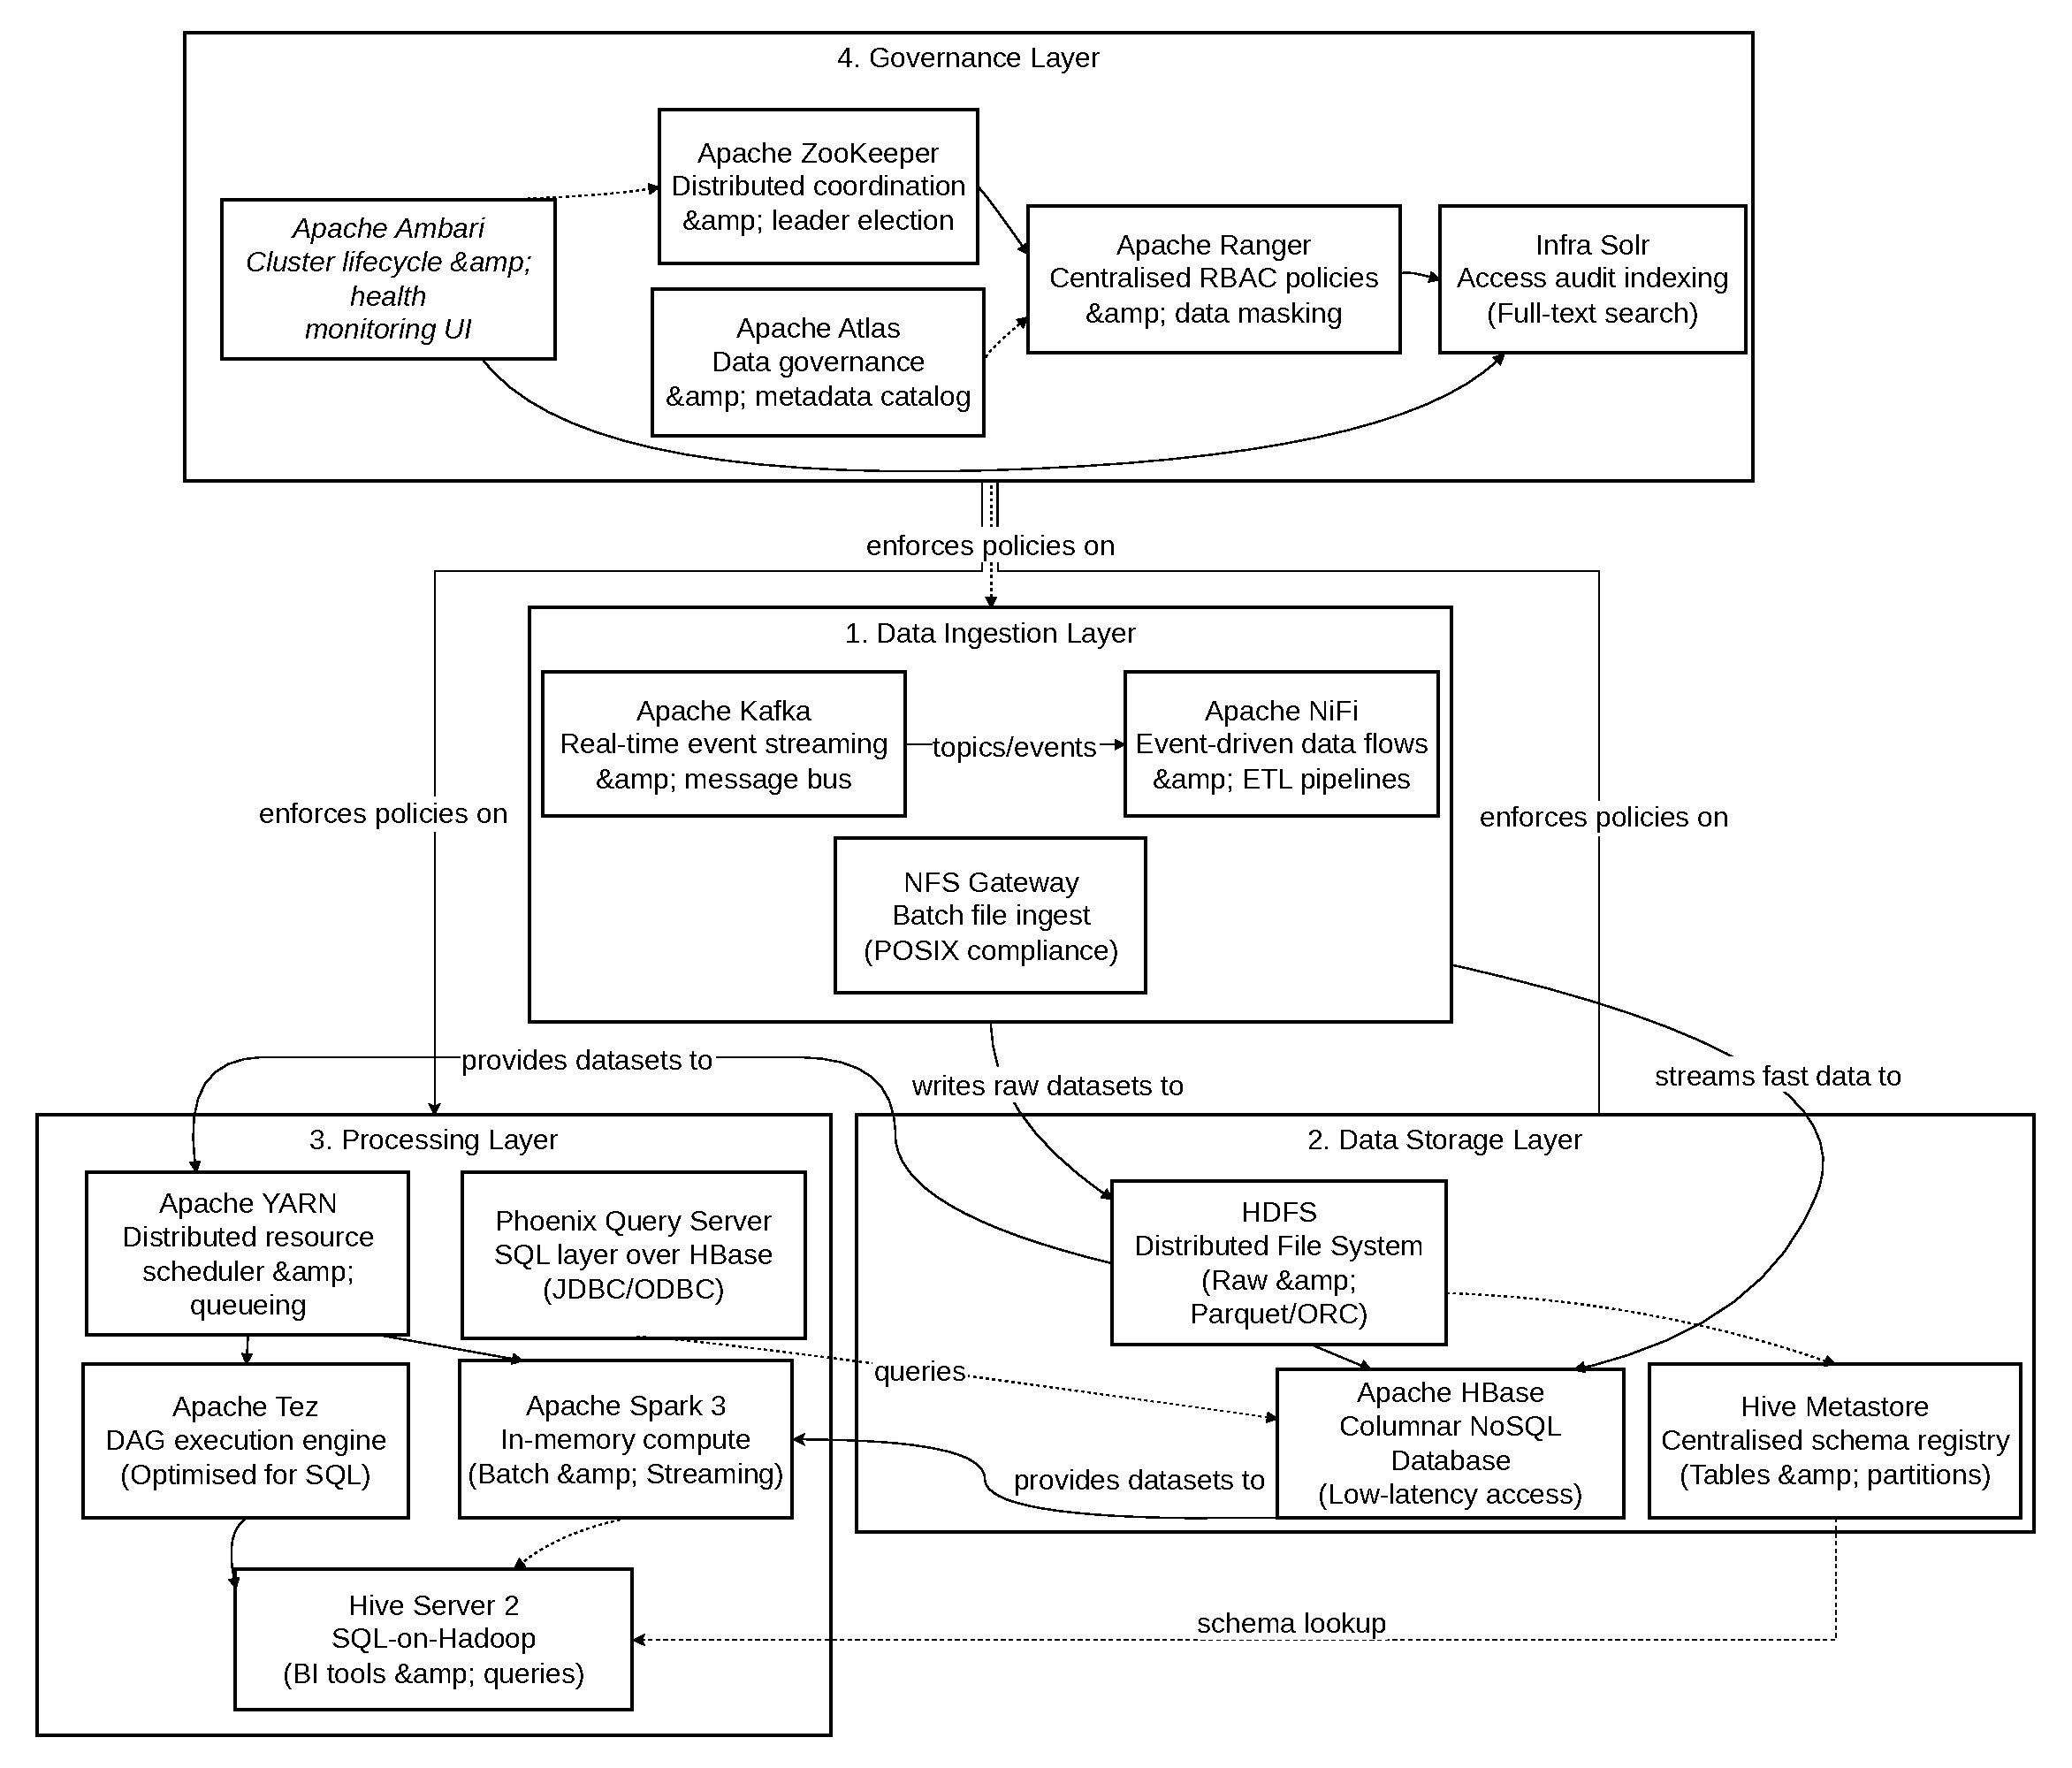
\includegraphics[width=\linewidth,height=0.78\textheight,keepaspectratio]{datalake-architecture.pdf}
\end{frame}

\begin{frame}{Perfis de instala\c{c}\~ao}{Benchmark no perfil \textit{data science}}
  \begin{itemize}
    \item \textbf{Default}: stack completo (ingest\~ao, HBase, Spark, Hive, Ranger, \ldots).
    \item \textbf{Data science}: foco em \textbf{Spark + Hive + HDFS/YARN}; omite NiFi/HBase/Phoenix para liberar RAM/CPU --- \textbf{usado na avalia\c{c}\~ao SSB}.
    \item \textbf{Software engineering}: fluxos NiFi/Kafka/HBase, sem motores anal\'iticos Spark/Hive.
  \end{itemize}
  \vspace{0.35em}
  \begin{cefetblock}{Tempo de implanta\c{c}\~ao} \\
    Orquestra\c{c}\~ao Ambari + downloads: da ordem de \textbf{tr\^es horas} no Free Tier (incluindo ciclos de recupera\c{c}\~ao, se necess\'ario).
  \end{cefetblock}
\end{frame}


\section{Avalia\c{c}\~ao experimental}
% Protocolo experimental (SSB)

\begin{frame}{Objetivo e cen\'ario de teste}
  \begin{itemize}
    \item Verificar se \textbf{Spark} supera \textbf{Hive} em consultas anal\'iticas sobre hardware ARM \textbf{extremamente limitado}.
    \item Medir se \textbf{cache em mem\'oria} no Spark melhora ou piora o tempo face ao Spark ``padr\~ao'' sobre YARN.
    \item Cluster no perfil \texttt{data-science}: HDFS, YARN, Hive Metastore, HiveServer2, Spark~3 (ODP~1.2.2.0, CentOS Stream~9 aarch64).
  \end{itemize}
\end{frame}

\begin{frame}{Dataset SSB (fator de escala 10)}
  \begin{itemize}
    \item \textbf{SSB} com \texttt{dbgen}; CSV para o HDFS via n\'o mestre.
    \item Cinco tabelas \textbf{externas} no Metastore (\texttt{OpenCSVSerde}) --- Hive e Spark partilham o mesmo esquema.
    \item Fato \texttt{lineorder.csv}: \textbf{$\sim$9{,}3~GB} (I/O e RAM cr\'iticos a 6~GB/n\'o).
  \end{itemize}
\end{frame}

\begin{frame}{Tr\^es configura\c{c}\~oes e m\'etricas}
  \begin{enumerate}
    \item \textbf{Hive}: execu\c{c}\~ao orientada a disco via motor nativo do Hive.
    \item \textbf{Spark (sem cache)}: leitura direta do HDFS, par\^ametros YARN por defeito.
    \item \textbf{Spark + cache}: tabelas materializadas em mem\'oria \textbf{e} par\^ametros expl\'icitos de mem\'oria, executores e shuffle (ver artigo).
  \end{enumerate}
  \vspace{0.35em}
  \begin{cefetalertblock}{Contagem de execu\c{c}\~oes}
    \textbf{14 consultas} $\times$ \textbf{10 repeti\c{c}\~oes} $\times$ \textbf{3 configura\c{c}\~oes} = \textbf{420} tempos de parede registados (sem descartar warm-up).
  \end{cefetalertblock}
\end{frame}

\begin{frame}[fragile]{Par\^ametros Spark (extrato)}
  \begin{lstlisting}[language=bash, gobble=0]
-- Spark padrao (resumo)
spark-sql --master yarn

-- Spark com cache (exemplo de linha de comando)
spark-sql --master yarn --num-executors 2 --executor-cores 1
  --driver-memory 512m --executor-memory 1g
  --conf spark.executor.memoryOverhead=256m
  --conf spark.memory.fraction=0.8
  --conf spark.sql.shuffle.partitions=48
  \end{lstlisting}
  \vspace{0.25em}
  {\scriptsize\color{cefetMuted}Dois executores: limite duro de CPU/containers no blueprint (1 vCPU por NodeManager; AM ocupa um contentor).}
\end{frame}


\section{Resultados}
% Resultados

\begin{frame}{Tempos m\'edios: Hive vs.\ Spark vs.\ Spark + cache}
  \begin{itemize}
    \item Spark \textbf{mais r\'apido que Hive} nas 14 consultas; diferen\c{c}a m\'edia da ordem de \textbf{centenas de segundos}/consulta.
    \item \textbf{Cache}: frequentemente \textbf{pior} quando o fato grande n\~ao cabe na RAM; ganhos em algumas consultas mais pesadas (ex.: Q3.2).
  \end{itemize}
  \vspace{0.15em}
  \begin{center}
    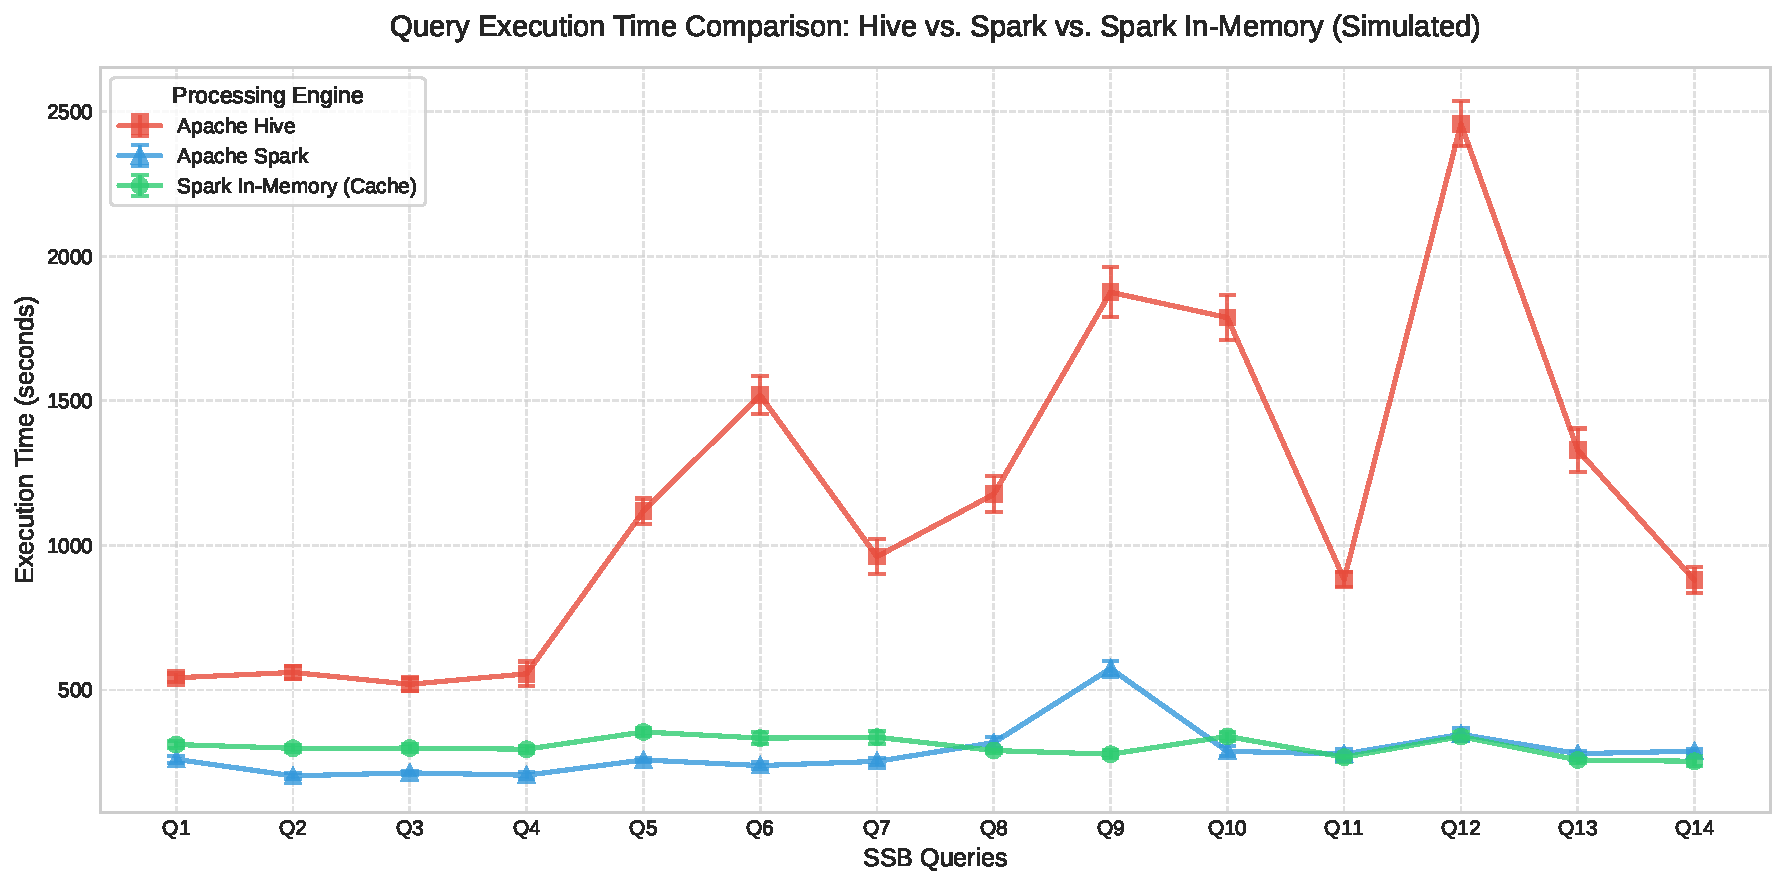
\includegraphics[width=0.95\linewidth,height=0.38\textheight,keepaspectratio]{graphic.pdf}
  \end{center}
\end{frame}

\begin{frame}{N\'umeros de refer\^encia (m\'edia em 10 execu\c{c}\~oes)}
  \footnotesize
  \centering
  \begin{tabular}{@{}lccc@{}}
    \rowcolor{cefetPrimary}
    \color{white}\bfseries Consulta
      & \color{white}\bfseries Hive (s)
      & \color{white}\bfseries Spark (s)
      & \color{white}\bfseries Spark+cache (s) \\
    \midrule
    \rowcolor{cefetBg}
    Q1.2a & 542 & 260 & 311 \\
    \rowcolor{cefetCodeBg}
    Q4.1 (pior Hive) & 2\,459 & 347 & 339 \\
    \rowcolor{cefetBg}
    Q3.2 (maior ganho cache) & 1\,872 & 575 & 278 \\
    \bottomrule
  \end{tabular}

  \vspace{0.65em}
  \begin{cefetexampleblock}{S\'intese}
    Margem m\'edia Hive$\rightarrow$Spark na ordem de \textbf{$\sim$868~s} por consulta; em m\'edia global, Spark+cache fica \textbf{$\sim$18~s mais lento} que Spark sem cache --- cache n\~ao compensa na maioria dos casos neste teto de mem\'oria.
  \end{cefetexampleblock}
\end{frame}


\section{Limita\c{c}\~oes e encerramento}
% Limitações e mensagem final

\begin{frame}{Limita\c{c}\~oes}
  \begin{itemize}
    \item Um \textbf{\'unico fator de escala} (SSB SF\,=\,10) e \textbf{topologia fixa} de 4 n\'os; sem \textbf{baseline x86} para isolar efeito da ISA.
    \item Spark ``padr\~ao'' vs.\ Spark+cache difere tamb\'em em \textbf{mem\'oria}, \textbf{fra\c{c}\~ao de mem\'oria Spark} e \textbf{parti\c{c}\~oes de shuffle} --- n\~ao \'e poss\'ivel atribuir o efeito s\'o ao cache.
    \item Teto de \textbf{4 OCPU / 24~GB} limita paralelismo e capacidade de cache; JVM/pacotes \textbf{ARM} podem comportar-se distinto de deployments x86 em produ\c{c}\~ao.
  \end{itemize}
\end{frame}

\begin{frame}{O que ficou demonstrado}
  \begin{itemize}
    \item \textbf{Execuções realizadas sem falhas irrecuper\'aveis }--- plataforma \textbf{est\'avel} sob stress prolongado no Free Tier.
    \item \textbf{Viabilidade pr\'atica} de anal\'itica distribu\'ida reprodut\'ivel com \textbf{custo monet\'ario nulo} de inst\^ancias, aceitando tempos mais longos e tuning cuidadoso.
  \end{itemize}
  \vspace{0.5em}
  \begin{cefetblock}{Mensagem central} \\
    Spark continua prefer\'ivel a Hive neste limite extremo de recursos; \textbf{estrat\'egias de cache} validadas em clusters maiores exigem \textbf{reavalia\c{c}\~ao} quando o fato principal n\~ao cabe na RAM agregada.
  \end{cefetblock}
\end{frame}


\cefetThanksFrame

\end{document}
